%______________________________________________________________________________________________________________________
% @brief    LaTeX2e Resume for Kamil K Wojcicki
\documentclass[margin,line]{resume}
\usepackage[colorlinks,urlcolor=blue]{hyperref}
\usepackage{fancyhdr}
\usepackage{pdflscape}
\usepackage{pdfpages}
\pagestyle{fancy}
\lhead{}
\chead{}
\rhead{}
\lfoot{}
\cfoot{Guo Yu - Page \thepage\ of 2}%
\rfoot{}
\renewcommand{\headrulewidth}{0pt}%
\renewcommand{\footrulewidth}{0pt}%

%______________________________________________________________________________________________________________________
\begin{document}
\name{
\Large{Yu Guo} ~ \small{(update: 02/01/2024)} 
~~~~~~~~~~~~~~
\href{https://tflsguoyu.github.io/}{\url{https://tflsguoyu.github.io/}}
~~~~~~~~~~~~~~~
\href{mailto:tflsguoyu@gmail.com}{tflsguoyu@gmail.com}
} 
\begin{resume}

    % %__________________________________________________________________________________________________________________
    % % Contact Information
    % \section{\mysidestyle Contact\\Information}

    % 4211 Donald Bren Hall                    \hfill \href{mailto:guo.yu@uci.edu}{guo.yu@uci.edu}  \\
    % University of California, Irvine                   \hfill \href{mailto:tflsguoyu@gmail.com}{tflsguoyu@gmail.com}\\
    % Irvine, CA 92697               \hfill \href{www.ics.uci.edu/~yug10}{\url{www.ics.uci.edu/~yug10}}
    
    %__________________________________________________________________________________________________________________
    % Current Position
    % \vspace{-5.0mm}
    % \line(1,0){440}
    % \vspace{-5.0mm}

    % \section{\mysidestyle Current Position}

    % \textbf{Tencent America} \hfill \textbf{CA \& NY, US}  \\
    % \textsl{Senior Graphics Researcher} \hfill 
    % \textbf{Sept. 2021 -- present} 

    %__________________________________________________________________________________________________________________
	% Research Interests
	\vspace{-5.0mm}
	\line(1,0){440}
	\vspace{-5.0mm}
	
	\section{\mysidestyle About Me}
	
	My background is mainly focused on \textbf{Computer Graphics}, specially in \textbf{Physics-based Rendering} and \textbf{Inverse-rendering}. I am also interested in \textbf{Material Capture and generation} by using \textbf{GAN/Diffusion} model. How to decompose \textbf{light/shadow} and material properties from a 3D model (Mesh/NeRF/\textbf{3DGS}) and make it \textbf{relightable} and \textbf{editable} are what I am willing to solve. Besides, I am interested in any project related to \textbf{Meta Human}.     

    %__________________________________________________________________________________________________________________
    % Education
    \vspace{-5.0mm}
    \line(1,0){440}
    \vspace{-5.0mm}

    \section{\mysidestyle Education}
    \textbf{University of California, Irvine}       \hfill \textbf{Irvine, CA, US}  \\
    \textsl{Ph.D in Computer Science} 															\hfill \textbf{Sept. 2016 -- Aug. 2021} \\
    \textbf{Dissertation}: Multi-scale Appearance Modeling of Complex Materials. \\
    \textbf{Advisor}: \href{https://shuangz.com/}{Shuang Zhao} 

    \textbf{University of Chinese Academy of Sciences}  \hfill \textbf{Beijing \& Shenzhen, China}\\
    \textsl{M.S. in Computer Science}                 \hfill \textbf{Sept. 2010 -- Jul. 2013} \\
	\textbf{Thesis}: GPU-based Soft Body Deformation with Nonlinear Finite Element Method. \\
	\textbf{Advisor}: \href{http://www.cse.cuhk.edu.hk/~pheng/}{Pheng Ann Heng} (CUHK)

    \textbf{Central South University}      \hfill \textbf{Changsha, China} \\
    \textsl{B.S. in Mathematics and Applied Mathematics}                \hfill \textbf{Sept. 2006 -- Jul. 2010}  \\
	\textbf{Thesis}: Forces Distribution with Fractal Theory in High Velocity Compaction Technology. \\
    
    %________________________________________________________________________________________________________________
    % Professional Experience
    \vspace{-5.0mm}
    \line(1,0){440}
    \vspace{-5.0mm}

    \section{\mysidestyle Working \\Experiences}

	\textbf{Tencent America} \hfill \textbf{New York \& Playa Vista, CA, US} \\
	\textsl{Senior Researcher at Pixel Lab, IEG} \hfill \textbf{Sept. 2021 -- Jan. 2024}\\
	\textbf{Working on} GenAI: diffusion model, 3D Gaussian splatting, image-based relighting; Unreal Engine 5: volumetric rendering; Photogrammetry: texture map delighting, shadow and highlight removal.\\
	\textbf{Manager}: \href{https://www.cs.columbia.edu/~cxz/}{Changxi Zheng} and  \href{https://sites.google.com/site/boyanghome/home}{Bo Yang}
	
	\vspace{0.0mm}

	\textbf{Facebook Reality Lab} \hfill \textbf{Sausalito, CA, US} \\
	\textsl{Research Intern at Monaco Team} \hfill \textbf{July. 2020 -- Sept. 2020}\\
	\textbf{Working on} Eye caustics rendering and its inverse problem.\\
	\textbf{Advisor}: \href{https://graphics.pixar.com/library/indexAuthorChristophe_Hery.html}{Christophe Hery}, \href{https://www.imdb.com/name/nm1436524/}{Olivier Maury}       

    \vspace{0.0mm}

	\textbf{Adobe Research} \hfill \textbf{San Jose, CA, US} \\
	\textsl{Research Intern at Emerging Graphics Group} \hfill \textbf{July. 2019 -- Sept. 2019}\\
	\textbf{Working on} Material capture and estimation.\\
	\textbf{Advisor}: \href{http://miloshasan.net/}{Milo\v{s} Ha\v{s}an}, \href{https://research.adobe.com/person/kalyan-sunkavalli/}{Kalyan Sunkavalli}       

    \vspace{0.0mm}

	\textbf{Megvii (Face++) Research USA} \hfill \textbf{Redmond, WA, US} \\
	\textsl{Research Intern} \hfill \textbf{July. 2018 -- Sept. 2018}\\
	\textbf{Working on} Human face shadow/highlight removal and face relighting.\\
	\textbf{Advisor}: \href{https://www.juew.org/}{Jue Wang}        

    \vspace{0.0mm}

    \textbf{Autodesk} \hfill \textbf{San Francisco, CA, US} \\
    \textsl{Research Intern at Core Rendering team} \hfill \textbf{July. 2017 -- Sept. 2017}\\
    \textbf{Working on} efficient volumetric rendering of 3D-printing materials.\\
    \textbf{Advisor}: \href{http://miloshasan.net/}{Milo\v{s} Ha\v{s}an}       
    
    \vspace{0.0mm}
    
    \textbf{Nanyang Technological University} \hfill \textbf{Singapore} \\
    \textsl{Research Associate at BeingThere Centre (\href{https://www.youtube.com/watch?v=Oy-xrxOB_4Q}{BTC}), IMI} \hfill \textbf{Oct. 2013 -- Mar. 2016}\\
    (BTC is a US\$18 million international research project on 3D Telepresence and Virtual Reality between ETH (\href{https://en.wikipedia.org/wiki/Markus_Gross}{Markus Gross}), UNC (\href{https://en.wikipedia.org/wiki/Henry_Fuchs}{Henry Fuchs}) and
    NTU (\href{https://en.wikipedia.org/wiki/Nadia_Magnenat_Thalmann}{Nadia Magnenat Thalmann}).)\\
    \textbf{Working on} stereo rendering; physical-based video manipulation; virtual try-on system for prescription glasses. \\
    \textbf{Collaborators}: \href{http://vrneurocog.wixsite.com/vrneurocog}{Miriam Reiner},
    \href{https://scholar.google.com/citations?user=XPZLx-8AAAAJ&hl=en}{Jean-Charles Bazin},
    \href{https://www.virtamed.com/en/about-us/team/tobias-martin-phd/}{Tobias Martin},
    \href{https://www.crunchbase.com/person/claudia-pluss}{Claudia Pl\"{u}ss},
    \href{http://www.py-laffont.info/}{Pierre-Yves Laffont},
    \href{https://qianzhanginfo.github.io/}{Qian Zhang} \\
    \textbf{Advisor}: \href{http://www.ntu.edu.sg/home/astjcham/}{Tat-Jen Cham} 

    \vspace{0.0mm}
    
    \textbf{Shenzhen Institutes of Advanced Technology}   \hfill \textbf{Shenzhen, China} \\
    \textsl{Research Assistant at HCI lab} \hfill \textbf{Sept. 2011 -- Jul. 2013} \\
    \textbf{Working on} mesh processing; soft body simulation; virtual surgery; CUDA acceleration. \\
    \textbf{Advisor}: Pheng-Ann Heng, Yongming Xie \\

    %__________________________________________________________________________________________________________________
	% Publications
	\vspace{-5.0mm}
	\line(1,0){440}
	\vspace{-5.0mm}
	
	\section{\mysidestyle Selected \\Publications}
	
	``\textbf{Woven Fabric Capture from a Single Photo}" 
	by Wenhua Jin, Beibei Wang, Milos Hasan, \textbf{Yu Guo}, Steve Marschner and Lingqi Yan. 
	\textsl{SIGGRAPH Asia '22}\\
	
	\vspace{-5mm}
	
	``\textbf{Beyond Mie Theory: Systematic Computation of Bulk Scattering Parameters based on Microphysical Wave Optics}" 
	by \textbf{Yu Guo}, Adrian Jarabo and Shuang Zhao. 
	\textsl{ACM Transactions on Graphics (TOG), 2021 (presented at SIGGRAPH Asia '21).}\\
	
	\vspace{-5mm}
	
	``\textbf{MaterialGAN: Reflectance Capture using a Generative SVBRDF Model}" 
	by \textbf{Yu Guo}, Cameron Smith, Milo\v{s} Ha\v{s}an, Kalyan Sunkavalli and Shuang Zhao. 
	\textsl{ACM Transactions on Graphics (TOG), 2020 (presented at SIGGRAPH Asia '20).}\\
	
	\vspace{-5mm}
	
	``\textbf{A Bayesian Inference Framework for Procedural Material Parameter Estimation}" 
	by \textbf{Yu Guo}, Milo\v{s} Ha\v{s}an, Lingqi Yan and Shuang Zhao. 
	\textsl{Computer Graphics Forum (CGF), 2020 (presented at Pacific Graphics '20).}\\
	
	\vspace{-5mm}
	
	``\textbf{Position-Free Monte Carlo Simulation for Arbitrary Layered BSDFs}" 
	by \textbf{Yu Guo}, Milo\v{s} Ha\v{s}an and Shuang Zhao. 
	\textsl{ACM Transactions on Graphics (TOG), 2018 (presented at SIGGRAPH Asia '18).}\\
	
	\vspace{-5mm}
	
	``\textbf{A Virtual Try-on System for Prescription Eyeglasses}" 
	by Qian Zhang, \textbf{Yu Guo}, Pierre-Yves Laffont, Tobias Martin, and Markus Gross. 
	\textsl{IEEE Computer Graphics and Applications (CG\&A), 2017.}\\
	
	\vspace{-5mm}
	
%	``\textbf{3D Faces are Recognized More Accurately and Faster than 2D Faces, but with Similar Inversion Effects}" 
%	by Derric Eng, Belle Yick, \textbf{Yu Guo}, Hong Xu, Miriam Reiner, Tat-Jen Cham, and Annabel Chen. 
%	\textsl{Vision Research, 2017.}\\
%	
%	\vspace{-5mm}
	
	``\textbf{Physically Based Video Editing}" 
	by Jean-Charles Bazin, Claudia Pl\"{u}ss (Kuster), \textbf{Yu Guo}, Tobias Martin, Alec Jacobson, and Markus Gross. 
	\textsl{Computer Graphics Forum (CGF), 2016 (presented at Pacific Graphics '16).}\\
	
	\vspace{-5mm}
	
%	``\textbf{GPU Accelerated CBCT Reconstruction from Few Views with SART and TV Regularization}" 
%	by Ping Liu, Lin Shi, Defeng Wang, \textbf{Yu Guo}, Jianying Li, Jing Qin, and Pheng-Ann Heng. 
%	\textsl{International Workshop on High Performance Computing for Biomedical Image Analysis (HPC-MICCAI), 2013.}\\
%	
%	\vspace{-5mm}
%	
%	``\textbf{Real-time Hand Detection Based on Multi-stage HOG-SVM Classifier}" 
%	by Jiang Guo, Jun Cheng, Jianxin Pang, and \textbf{Yu Guo}. 
%	\textsl{International Conference on Image Processing (ICIP), 2013.}\\
%	
%	\vspace{-5mm}
	
	``\textbf{A GPU-Accelerated Finite Element Solver for Simulation of Soft-Body Deformation}" 
	by \textbf{Yu Guo}, Jianying Li, Ping Liu, Qiong Wang, and Jing Qin. 
	\textsl{International Conference on Information and Automation (ICIA), 2013.}\\
	
	\vspace{-5mm}
	
%	``\textbf{A Survey on Simulation of Soft Tissue Deformation in Virtual Surgery}(In Chinese)" 
%	by \textbf{Yu Guo}, Jing Qin. 
%	\textsl{Journal of Integration Technology (JIT), 2013.}\\
%	
%	\vspace{-5mm}
%	
%	``\textbf{Fall over or Sliding down?}" 
%	by \textbf{Yu Guo}.
%	\textsl{SIGGRAPH Asia (Poster), 2012.}\\
%	
%	\vspace{-5mm}
	
	``\textbf{A Master-Slave Robotic Simulator Based on GPUDirect}" 
	by Jianying Li, \textbf{Yu Guo}, Heye Zhang, Yongming Xie.
	\textsl{International Conference on Intelligent Robots and Systems (IROS), 2012.}\\

    %__________________________________________________________________________________________________________________
    % Honours and Awards
    % \vspace{-5.0mm}
    % \line(1,0){440}
    % \vspace{-5.0mm}

    % \section{\mysidestyle Awards}

    % 2nd class prize in 4th \textsl{ACM CSU Collegiate Programming Contest}. ~ CSU, China    \hfill 2010      \\
    % 1st class prize in 3rd \textsl{CSU Mathematical Contest in Modeling}. ~ CSU, China      \hfill 2008      \\
    % 1st class prize in National High School Student Mathematics Competition. ~ China        \hfill 2005      \\


    %__________________________________________________________________________________________________________________
    % Professional activities
    \vspace{-5.0mm}
    \line(1,0){440}
    \vspace{-5.0mm}

    \section{\mysidestyle Reviews}

    TOG, CGF, SIGGRAPH, SIGGRAPH Asia, EG, PG                    \\


    %__________________________________________________________________________________________________________________
    % Computer Skills
    % \vspace{-5.0mm}
    % \line(1,0){440}
    % \vspace{-5.0mm}

    % \section{\mysidestyle Computer \\Skills}

    % \textbf{Programming Tools:} C++, Python, MATLAB \\
    % \textbf{Others:} Mitsuba, PyTorch, \LaTeX  \\                                 


%______________________________________________________________________________________________________________________
\end{resume}

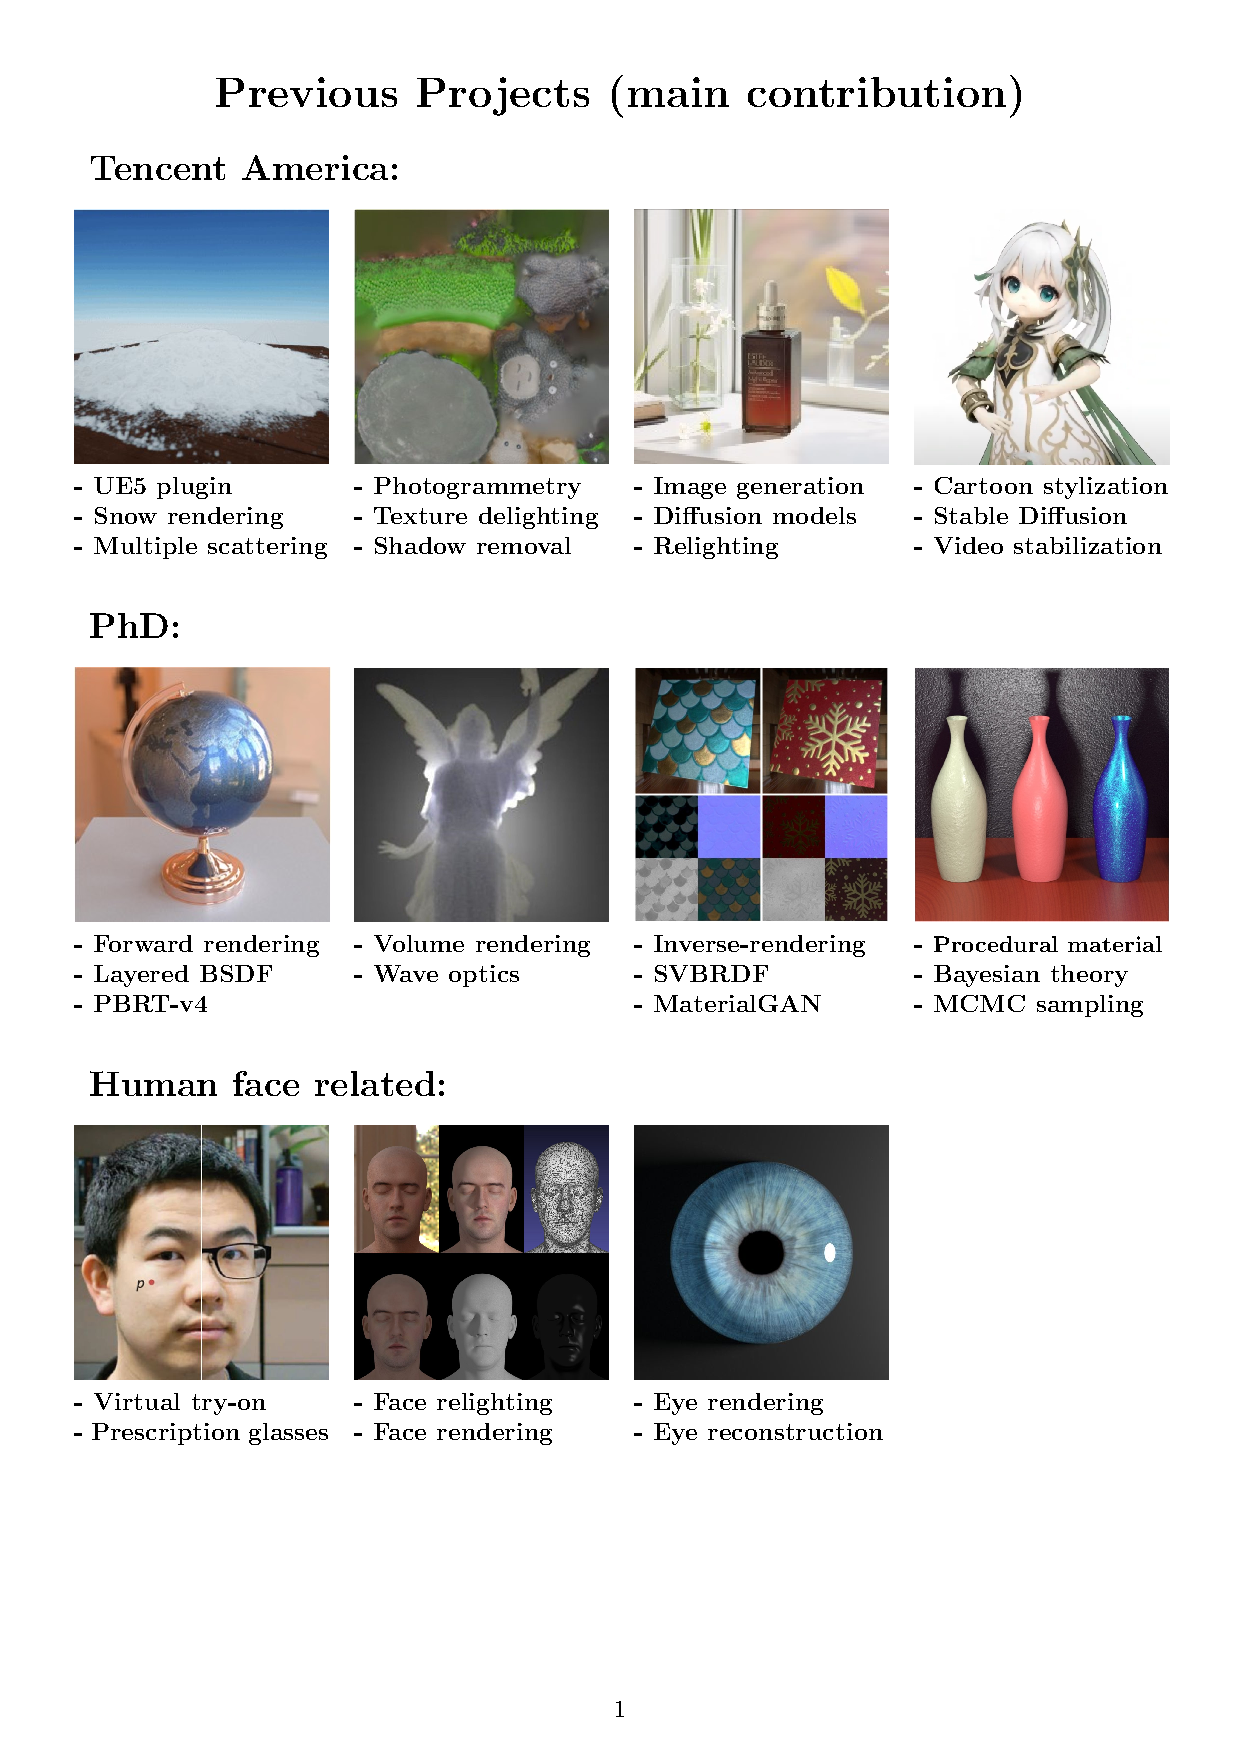
\includepdf[pages=1, scale=1.05, angle=0,  offset=-1.1in -0.5in]{fig/projects.pdf}

\end{document}
%______________________________________________________________________________________________________________________
% EOF

